% fig1_silent_decision_problem.tex — Figure 2 (column width)
% Runtime audit (status quo) vs. compile-time guarantee (BTV).
% Regenerated 2026-09-15 (COMSI-2026-04-0112 R1), monochrome.
% Redesign 2026-09-15 (design/ieee-figure-redesign): panel headers moved
% to explicit nodes ABOVE each bordered panel (not corner labels on the
% fit box) — the corner-label mechanism let panel B's header overlap the
% EvidenceToken box; explicit stacked nodes remove the ambiguity.
\documentclass[border=2pt]{standalone}
\usepackage{tikz}
\usetikzlibrary{arrows.meta,positioning,fit,calc,shapes.misc}
\usepackage{amssymb}
\begin{document}
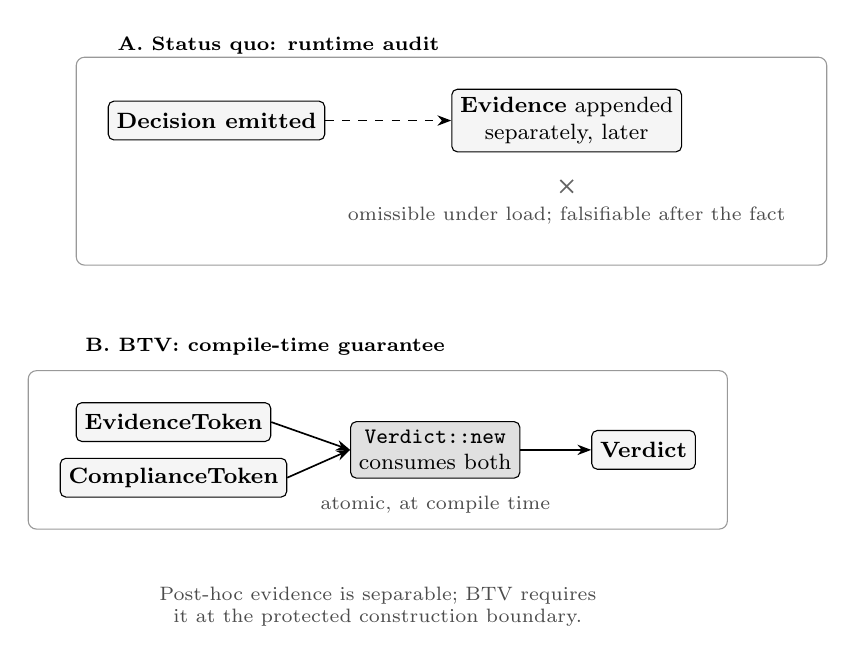
\begin{tikzpicture}[
  font=\footnotesize,
  box/.style={draw, rounded corners=2pt, align=center, inner sep=3pt,
    minimum height=14pt, fill=black!04},
  arr/.style={-{Stealth[length=5pt]}, semithick},
  lost/.style={-{Stealth[length=5pt]}, semithick, dashed},
  note/.style={align=center, font=\scriptsize, text=black!70},
  hdr/.style={font=\scriptsize\bfseries, align=left},
  panel/.style={draw=black!40, rounded corners=3pt, inner sep=4mm}
]

% ── Panel A: status quo ──────────────────────────────────────────────────
\node[hdr] (hA) at (0,0) {A. Status quo: runtime audit};
\node[box, below=7mm of hA.west, anchor=north west] (dec) {\textbf{Decision emitted}};
\node[box, right=16mm of dec] (evd) {\textbf{Evidence} appended\\ separately, later};
\draw[lost] (dec) -- (evd);
\node[draw=black!60, cross out, semithick, below=3.5mm of evd, inner sep=2pt] (x) {};
\node[note, below=1.5pt of x] (xnote) {omissible under load; falsifiable after the fact};
\node[panel, fit=(dec)(evd)(x)(xnote)] (p1) {};

% ── Panel B: BTV ──────────────────────────────────────────────────────────
\node[hdr, below=8mm of p1.south west, anchor=north west] (hB) {B. BTV: compile-time guarantee};
\node[box, below=7mm of hB.west, anchor=north west] (tokE) {\textbf{EvidenceToken}};
\node[box, below=2mm of tokE] (tokC) {\textbf{ComplianceToken}};
\node[box, right=9mm of $(tokE.east)!0.5!(tokC.east)$, fill=black!12] (cons)
  {\texttt{Verdict::new}\\ consumes both};
\node[box, right=9mm of cons] (verd) {\textbf{Verdict}};
\draw[arr] (tokE.east) -- ($(cons.west)!0.65!(cons.west)$);
\draw[arr] (tokC.east) -- ($(cons.west)!0.35!(cons.west)$);
\draw[arr] (cons) -- (verd);
\node[note, below=1mm of cons] {atomic, at compile time};
\node[panel, fit=(tokE)(tokC)(cons)(verd)] (p2) {};

% ── synthesis line ───────────────────────────────────────────────────────
\node[note, below=6mm of p2.south, text width=68mm, align=center]
  {Post-hoc evidence is separable; BTV requires it at the protected construction boundary.};

\end{tikzpicture}
\end{document}
